The MiniMax algorithm is a decision rule algorithm for minimizing the possible
loss for a worst case (maximum loss) scenario in a zero sum game for 2 (or more)
players who play in turns.

The algorithm builds a game tree, where each tree node represents a game state
and the children represent the possible game moves that can be made by either
player 1 or player 2.  An evaluation function is used to compute the score of
the game for each leaf of the tree. A node is a leaf when the game state can no
longer be expanded. Finally, the algorithm recursively minimizes or maximizes
the scores of each node. To select the best move for player 1, the algorithm
picks the move maximized at the root node.

In LM, the program starts with a root node (with the initial game state) that
is expanded with the available moves at each level. The graph of the program is
dynamic since nodes are created and then deleted once they are no longer
needed. The latter happens when the leaf scores are computed or when a node
fully minimizes or maximizes the children scores. When the program ends, only
the root node has facts in its database.

The full MiniMax code is shown in Fig.~\ref{code:coord:minimax}. The first two
rules in lines~\ref{line:coord:minimax_play1}-\ref{line:coord:minimax_play2}
check if the current game is final, namely, if a player has won or the game
drew: the first rule generates the score for the final state while the second
expands the game state by generating all the possible plays for player
\code{NextPlayer}.

The expansion rules creates the children for the current node and are
implemented in
lines~\ref{line:coord:minimax_expand1}-\ref{line:coord:minimax_expand2}. The
first two rules create either a \code{maximize} or \code{minimize} fact that
will either maximize or minimize the scores of the children nodes.  The third
and fourth expansion rules simulate a player move and, for that, create a new
node \code{B} using the \code{exists} language construct. We link \code{B} with
\code{A} using \code{parent(B, A)} and kickstart the recursive expansion of node
\code{B} by deriving a \code{play} fact. Finally, the rule in
lines~\ref{line:coord:minimax_expand11}-\ref{line:coord:minimax_expand2} is for
the case when the current player cannot play in the current game position.

\begin{wrapfigure}{r}{0.4\textwidth}
   \begin{center}
      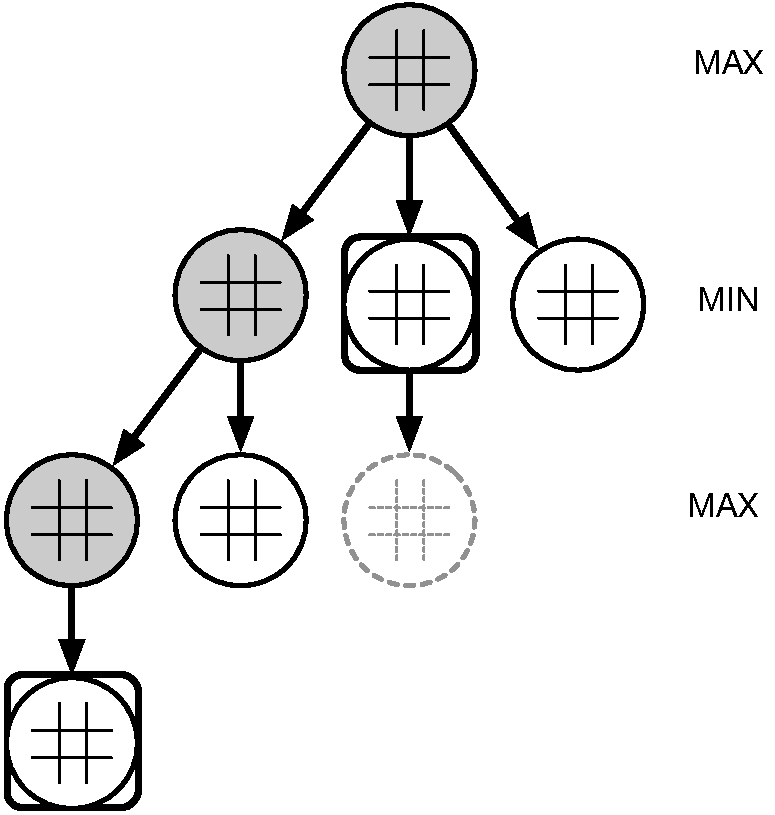
\includegraphics[width=0.9\linewidth]{figures/coordination/minimax_tree}
   \end{center}
   \caption{Expanding the MiniMax tree using coordination. By prioritizing
      deeper nodes, threads are forced to expand the tree using a depth-first
      approach, which is superior since there is no need to expand the whole
      tree before computing the node scores.}
   \label{fig:coord:minimax}
\end{wrapfigure}

As noted in Section~\ref{sec:coord:fifo}, the default scheduler uses a FIFO
approach, which results in a breadth-first search on the MiniMax tree. This
results in $\mathcal{O}(n)$ space complexity, where $n$ is the number of nodes
in the tree, since the tree must be fully expanded before the scores at the
leaves are actually computed.  With coordination, we set the priority of a node
to be its depth (lines~\ref{line:coord:minimax_coord1} and
\ref{line:coord:minimax_coord2}) so that the tree is expanded in a depth-first
fashion, leading to $\mathcal{O}(d t)$ memory complexity, where $d$ is the depth
of the tree and $t$ is the number of threads. Since threads prioritize deeper
nodes, the scores of the first leaves are immediately computed and then sent to
the parent node. At this point, the leaves are deleted and reused for other
nodes in the tree, resulting in minimal memory usage.  As an example, consider a
system with 2 threads, $T_1$ and $T_2$, where $T_1$ first expands the root node
and then the first child. Since $T_2$ is idle, it steals half of the root's
children nodes and starts expanding one of the nodes in a depth-first fashion.

\begin{figure}[ht]
\begin{Verbatim}[numbers=left,commandchars=\\\{\},fontsize=\codesize]
type list int game.
type linear parent(node, node).
type linear score(node, int, int). type linear new-score(node, int, int).
type linear minimize(node, int, int, int). type linear maximize(node, int, int, int).
type linear expand(node, game FirstPart, game SecondPart,
   int Descendants, int Player, int Play, int Depth).
type linear play(node, game Game, int Player, int Play, int Depth).

const root-player = 1. const initial-game = [...].
fun next(P : int) : int = if P = 1 then 2 else 1 end.

play(@0, initial-game, root-player, 0, 1).\label{line:coord:minimax_axiom}

play(A, Game, NextPlayer, LastPlay, Depth),\label{line:coord:minimax_play1}\label{line:coord:minimax_play11}
Score = minimax_score(Game, NextPlayer, root-player), Score > 0
   -o score(A, Score, LastPlay).\label{line:coord:minimax_play12}
play(A, Game, NextPlayer, LastPlay, Depth),\label{line:coord:minimax_play21}
0 = minimax_score(Game, NextPlayer, root-player)
   -o expand(A, [], Game, 0, NextPlayer, LastPlay, Depth).\label{line:coord:minimax_play2}\label{line:coord:minimax_play22}

expand(A, Game, [], N, Player, Play, \underline{Depth}), Player = root-player\label{line:coord:minimax_expand1}\label{line:coord:minimax_rule11}
   -o maximize(A, N, -00, 0).\label{line:coord:minimax_rule12}
expand(A, Game, [], N, Player, Play, \underline{Depth}), Player <> root-player\label{line:coord:minimax_rule21}
   -o minimize(A, N, +00, 0).\label{line:coord:minimax_rule22}
expand(A, First, [0 | Xs], N, Player, Play, \underline{Depth}), Depth >= 5\label{line:coord:minimax_rule31}
   -o exists B. (\underline{set-static(B)},\label{line:coord:minimax_coord1}
       \underline{set-default-priority(B, float(Depth + 1))},\label{line:coord:minimax_coord2}
       play(B, Game ++ [P | Xs], next(P), length(First), \underline{Depth + 1}), parent(B, A).
       expand(A, First ++ [0], Xs, N + 1, Player, Play, \underline{Depth})).\label{line:coord:minimax_rule32}
expand(A, First, [0 | Xs], N, Player, Play, \underline{Depth}), Depth < 5\label{line:coord:minimax_rule41}
  -o exists B. (\underline{set-default-priority(B, float(Depth + 1))},\label{line:coord:minimax_coord3}
       play(B, Game ++ [P | Xs], next(P), length(First), \underline{Depth + 1}), parent(B, A),
       expand(A, First ++ [0], Xs, N + 1, Player, Play, \underline{Depth})).\label{line:coord:minimax_rule42}
expand(A, First, [C | Xs], N, Player, Play, \underline{Depth}) C <> 0\label{line:coord:minimax_expand11}\label{line:coord:minimax_rule51}
  -o expand(A, First ++ [C], Xs, N, Player, Play, \underline{Depth}).\label{line:coord:minimax_expand2}\label{line:coord:minimax_rule52}

score(A, Score, BestPlay), parent(A, B) -o new-score(B, Score, BestPlay).\label{line:coord:minimax_new}

new-score(A, Score, Play), minimize(A, N, Current, BestPlay), Current > Score\label{line:coord:minimax_minimize1}
   -o minimize(A, N - 1, Score, Play).
new-score(A, Score, Play), minimize(A, N, Current, BestPlay), Current <= Score
   -o minimize(A, N - 1, Current, BestPlay).
minimize(A, 0, Score, BestPlay) -o score(A, Score, BestPlay).\label{line:coord:minimax_minimize2}

new-score(A, Score, Play), maximize(A, N, Current, BestPlay), Current < Score\label{line:coord:minimax_maximize1}\label{line:coord:minimax_maximize_rule11}
   -o maximize(A, N - 1, Score, Play).\label{line:coord:minimax_maximize_rule12}
new-score(A, Score, Play), minimize(A, N, Current, BestPlay), Current >= Score\label{line:coord:minimax_maximize_rule21}
   -o maximize(A, N - 1, Current, BestPlay).\label{line:coord:minimax_maximize_rule22}
maximize(A, 0, Score, BestPlay) -o score(A, Score, BestPlay).\label{line:coord:minimax_maximize2}
\end{Verbatim}
\caption{LM code for the MiniMax program.}
\label{code:coord:minimax}
\end{figure}

We also take advantage of memory locality by using \code{set-static}
(line~\ref{line:coord:minimax_coord2}), so that nodes after a certain level are
   not stolen by other threads. While this is not critical for performance in
   shared memory systems where node stealing is fairly efficient, we expect that
   such coordination to be critical in distributed systems.

The rest of the program contains rules for maximizing and minimizing scores
(lines~\ref{line:coord:minimax_minimize1}-\ref{line:coord:minimax_maximize2}),
through the retraction of \code{new-score} incoming facts.

\begin{figure}[ht]
   \begin{center}
      \begin{tabular}[b]{ | c | c | c |}
         \hline
         \textbf{\# T} & \textbf{Reg} & \textbf{Coord} \\ \hline \hline
         1 & 4.85GB & 0.38MB \\ \hline
         2 & 5.29GB & 0.65MB \\ \hline
         4 & 5.88GB & 1.28MB \\ \hline
         8 & 5.66GB & 2.42MB \\ \hline
         16 & 5.04GB & 4.68MB \\ \hline
         \end{tabular}
   \end{center}

   \caption{(a) Memory usage and (b) scalability of the regular and coordinated
versions of MiniMax.}
   \label{results:memory_minmax}
\end{figure}

In Fig.~\ref{results:memory_minmax} we compare the memory usage and scalability
of the coordinated MiniMax against the regular MiniMax. The coordinated version
uses significantly less memory (at most 4.68MB for 16 threads) than the regular
version (around 5.04GB). Note that as the number of threads goes up, memory
usage also goes up. This is an artifact of our parallel memory allocator that
allocates large chunks of memory beforehand. In terms of scalability, our
experimental results show that the coordinated version running on 16 threads is
almost 4 times faster than the hand-written sequential C program, while the
regular version is barely as fast as the same C program. XXX

\subsubsection{Proof of correctness}

To prove that the MiniMax code shown in Fig.~\ref{code:coord:minimax} computes
the best score along with the best possible move that the \code{root-player} can
make, we have to generalize the proof and inductively prove that each node
selects the best score depending if its a minimizing or a maximizing node. We
start with several useful lemmas.

\begin{lemma}[Play Lemma]

If \code{expands(A, FirstGame, RestGame, NumberDescendants, NextPlayer, Play,
Depth)} then $\exists_n$ where $n$ is the number of available plays that
\code{NextPlayer} can make on the remaining game state \code{RestGame}.  We also
create $n$ children $B$ where \code{play(B, Game', OtherPlayer, Play', Depth +
1)} and \code{parent(B, A)} is true, where \code{OtherPlayer =
next-player(NextPlayer)}, \code{Play'} is the index of an empty position in
\code{RestGame} plus the length of \code{FirstGame}, and \code{Game'} represents
the concatenation of \code{FirstGame} and \code{RestGame} where an empty
position has been modified. Eventually, \code{expands} disappear and if
\code{NextPlayer = root-player}, \code{maximize(A, NumberDescendants + Empty,
mininf, 0)} or \code{minimize(A, NumberDescendants + Empty, maxinf, 0)},
respectively. The value \code{Empty} indicates the number of empty positions in
the state \code{RestGame}.

\end{lemma}

\begin{proof}
By induction on the size of the list \code{RestGame}. There are 5 possible rules.

Rule 1 (lines~\ref{line:coord:minimax_rule11}-\ref{line:coord:minimax_rule12}:
\code{RestGame = []} thus a \code{maximize} fact is derived as expected.

Rule 2 (lines~\ref{line:coord:minimax_rule21}-\ref{line:coord:minimax_rule22}:
\code{RestGame = []} thus a \code{minimize} fact is derived as expected.

Rule 3 (lines~\ref{line:coord:minimax_rule31}-\ref{line:coord:minimax_rule32}:
in this case we have a non-null \code{RestGame} and an empty position on index
0. As expected, we create a new \code{B} node with the right facts and a new
\code{expand} fact with a smaller \code{RestGame}. Apply the induction
hypothesis to get the remaining $n-1$ potential plays for \code{NextPlayer}.

Rule 4 (lines~\ref{line:coord:minimax_rule41}-\ref{line:coord:minimax_rule42}:
same reasoning as rule 3. Note that the presence of coordination facts do not
change the proof because they are not used in the rule's LHS.

Rule 5 (lines~\ref{line:coord:minimax_rule51}-\ref{line:coord:minimax_rule52}:
no free space on the first position of \code{RestGame}. We derive another
\code{expand} fact with a reduced \code{RestGame} and use the induction
hypothesis.

\end{proof}

\begin{lemma}[Children Lemma]
If \code{play(A, Game, NextPlayer, LastPlay, Depth)} then either \code{score(A, Score,
      LastPlay)} or $\exists_n$ where $n$ is the number of available plays for
\code{NextPlayer} in \code{Game}, creating $n$ new children $B$ where \code{play(B,
      Game', OtherPlayer, Play, Depth + 1)} and a \code{maximize(A, N,
         mininf, 0)} or \code{minimize(A, N, maxinf, 0)} is created if
         $NextPlayer = root-player$ or not, respectively. \code{Game'} is an
         updated \code{Game} state where an empty position is played by
         \code{NextPlayer}.
\end{lemma}
\begin{proof}

A linear fact \code{play(A, Game, NextPlayer, LastPlay, Depth)} can only be used
in either in the first or second rules.
If the rule in
lines~\ref{line:coord:minimax_play11}-\ref{line:coord:minimax_play12} executes,
(\code{minimax\_score} returns a score) it means that \code{Game} is a final
game state and there's no available plays for \code{NextPlayer}.
Otherwise, the second rule in
lines~\ref{line:coord:minimax_play21}-\ref{line:coord:minimax_play22} will
apply and the Play lemma is used to prove this lemma.

\end{proof}

We now prove that the minimization and maximization rules work given the right
amount of scores available.

\begin{lemma}[Maximize Lemma]
Given a fact \code{maximize(A, N, BestScore, BestPlay)} and \code{N} facts
\code{new-score(A, OtherScore, OtherPlay)}, then we end up with a single
\code{score(A, BestScore', BestPlay')} where \code{BestScore'} is the
highest score from \code{BestScore} or \code{OtherScore'}s and
\code{BestPlay'} is the corresponding play.
\end{lemma}
\begin{proof}
By induction on the number of \code{new-score} facts.

Case 1 (\code{N = 0}): trivial by applying the rule in
line~\ref{line:coord:minimax_maximize2}.

Case 2 (\code{N > 0}): by picking an arbitrary \code{new-score(A, OtherScore,
OtherPlay} fact.

\begin{itemize}
   \item Sub case 2.1
      (lines~\ref{line:coord:minimax_maximize_rule11}-\ref{line:coord:minimax_maximize_rule12})

      If \code{BestScore < OtherScore} then we derive \code{maximize(A, N-1,
      OtherScore, OtherPlay)}. Use induction to get the final \code{score} fact.

   \item Sub case 2.2
      (lines~\ref{line:coord:minimax_maximize_rule21}-\ref{line:coord:minimax_maximize_rule22})

      If \code{BestScore >= OtherScore} then we derive \code{maximize(A, N-1,
      BestScore, BestPlay)}. Use induction to get the final \code{score} fact.

\end{itemize}

\end{proof}

\begin{lemma}[Minimize Lemma]
Given a fact \code{minimize(A, N, BestScore, BestPlay)} and \code{N} facts
\code{new-score(A, OtherScore, OtherPlay)}, then we end up with a single
\code{score(A, BestScore', BestPlay')} where \code{BestScore'} is the
lowest score from either \code{BestScore} or \code{OtherScore'}s and
\code{BestPlay'} is the corresponding play.
\end{lemma}
\begin{proof}
Use the same process used in Maximize Lemma.
\end{proof}

Finally, we are in a position to prove that a \code{play} fact eventually
produces a \code{score} fact that indicates the best score and best play for the
player playing at that node.

\begin{theorem}[Score Theorem]
For every \code{play(A, Game, NextPlayer, LastPlay, Depth)}, we either
directly get a \code{score} fact (leaf case) or a recursive alternate maximization or
minimization (depending if \code{NextPlayer = root-player}, respectively) of
the children nodes. This max/minization also results in a \code{score(A, Score,
BestPlay)} fact where \code{Score} is the max/minimum and \code{BestPlay} is the
corresponding play for that score.
\end{theorem}
\begin{proof}
By applying the Children Lemma and using induction on the number of free
positions on the state \code{Game}.

Case 1 (no free positions or game is final): direct score.

Case 2 (available positions): $n$ children nodes $B$ with \code{play(B, Game',
next-player(NextPlayer), X, Play, Depth + 1)}, where \code{Game'} has position
\code{X} filled up. We apply induction on the \code{play} fact of each child
\code{B} to get a \code{score(B, Score, Play)}. Since we also derived a
\code{parent(B, A)} fact, rule in line~\ref{line:coord:minimax_new} eventually
executes, deriving \code{new-score(A, Score, Play)}.

Since we also derived \code{maximize(A, N, mininf, 0)} (or \code{minimize}), we
have this maximize fact and $n$ \code{new-score} facts from the $n$ children
nodes. Applying the Maximize Lemma, we get \code{score(A, BestScore, BestPlay)}.

\end{proof}

\begin{corollary}[MiniMax]
Starting from a \code{play(@0, initial-game, root-player, 0, 1)}, the fact
\code{score(A, BestScore, BestPlay)} is eventually derived, where \code{BestPlay} represents the
best play which player \code{root-player} is able to make that minimizes the possible loss for
a worst case scenario giving \code{initial-game}.
\end{corollary}
\clearpage
